% The plane F_3^2: lines and a cap. Generated by a short script.
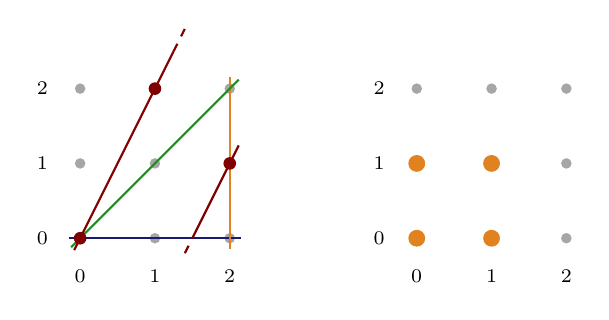
\begin{tikzpicture}[scale=0.95]
\fill[black!35] (0,0) circle (2pt);
\fill[black!35] (0,1) circle (2pt);
\fill[black!35] (0,2) circle (2pt);
\fill[black!35] (1,0) circle (2pt);
\fill[black!35] (1,1) circle (2pt);
\fill[black!35] (1,2) circle (2pt);
\fill[black!35] (2,0) circle (2pt);
\fill[black!35] (2,1) circle (2pt);
\fill[black!35] (2,2) circle (2pt);
\node[font=\scriptsize,below] at (0,-0.3) {$0$};
\node[font=\scriptsize,left] at (-0.3,0) {$0$};
\node[font=\scriptsize,below] at (1,-0.3) {$1$};
\node[font=\scriptsize,left] at (-0.3,1) {$1$};
\node[font=\scriptsize,below] at (2,-0.3) {$2$};
\node[font=\scriptsize,left] at (-0.3,2) {$2$};
\draw[MidnightBlue,thick] (-0.15,0) -- (2.15,0);
\draw[BurntOrange!90!black,thick] (2,-0.15) -- (2,2.15);
\draw[ForestGreen,thick] (-0.12,-0.12) -- (2.12,2.12);
\draw[Maroon,thick] (-0.08,-0.16) -- (1.25,2.5);
\draw[Maroon,thick,dashed] (1.25,2.5) -- (1.4,2.8);
\draw[Maroon,thick,dashed] (1.4,-0.2) -- (1.5,0);
\draw[Maroon,thick] (1.5,0) -- (2.12,1.24);
\fill[Maroon] (0,0) circle (2.4pt);
\fill[Maroon] (1,2) circle (2.4pt);
\fill[Maroon] (2,1) circle (2.4pt);
\fill[black!35] (4.5,0) circle (2pt);
\fill[black!35] (4.5,1) circle (2pt);
\fill[black!35] (4.5,2) circle (2pt);
\fill[black!35] (5.5,0) circle (2pt);
\fill[black!35] (5.5,1) circle (2pt);
\fill[black!35] (5.5,2) circle (2pt);
\fill[black!35] (6.5,0) circle (2pt);
\fill[black!35] (6.5,1) circle (2pt);
\fill[black!35] (6.5,2) circle (2pt);
\node[font=\scriptsize,below] at (4.5,-0.3) {$0$};
\node[font=\scriptsize,left] at (4.2,0) {$0$};
\node[font=\scriptsize,below] at (5.5,-0.3) {$1$};
\node[font=\scriptsize,left] at (4.2,1) {$1$};
\node[font=\scriptsize,below] at (6.5,-0.3) {$2$};
\node[font=\scriptsize,left] at (4.2,2) {$2$};
\fill[BurntOrange!90!black] (4.5,0) circle (3.2pt);
\fill[BurntOrange!90!black] (4.5,1) circle (3.2pt);
\fill[BurntOrange!90!black] (5.5,0) circle (3.2pt);
\fill[BurntOrange!90!black] (5.5,1) circle (3.2pt);
\end{tikzpicture}
